\section{Experiments}
\label{sec:experiment}

%In this section, we compare the proposed PU-GAN quantitatively and qualitatively with state-of-the-art point upsampling methods, and evaluate various aspects of our model. Please refer to the supplementary for extended experiments. Upon publication, we will release the full training and test data set, as well as the trained network and source code.
%for further implementation details

\begin{figure*}[t]
	\centering
	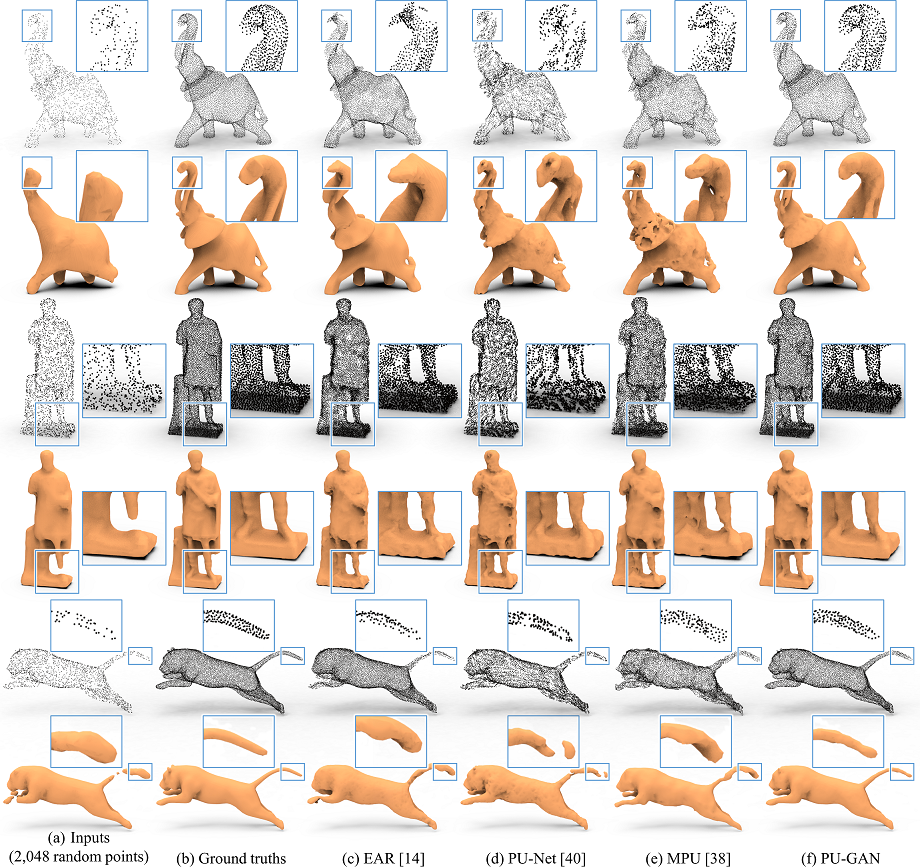
\includegraphics[width=0.99\linewidth]{visualComparison}
	\caption{Comparing point set upsampling (x4) and surface reconstruction results produced with different methods (c-f) from inputs (a).}
%	\caption{Comparing the point set upsampling results and the mesh reconstruction results produced using different methods (c-f) from inputs (a) with 2,048 non-uniform points.}
	\label{fig:visualComparison}
	\vspace*{-2mm}
\end{figure*}

%%%%%%%%%%%%%%%%%%%%%%%%%%%%%%%%%%%%%%%%%%%%%%%%%%%%%%%%%%%

\begin{figure*}[t]
	\centering
	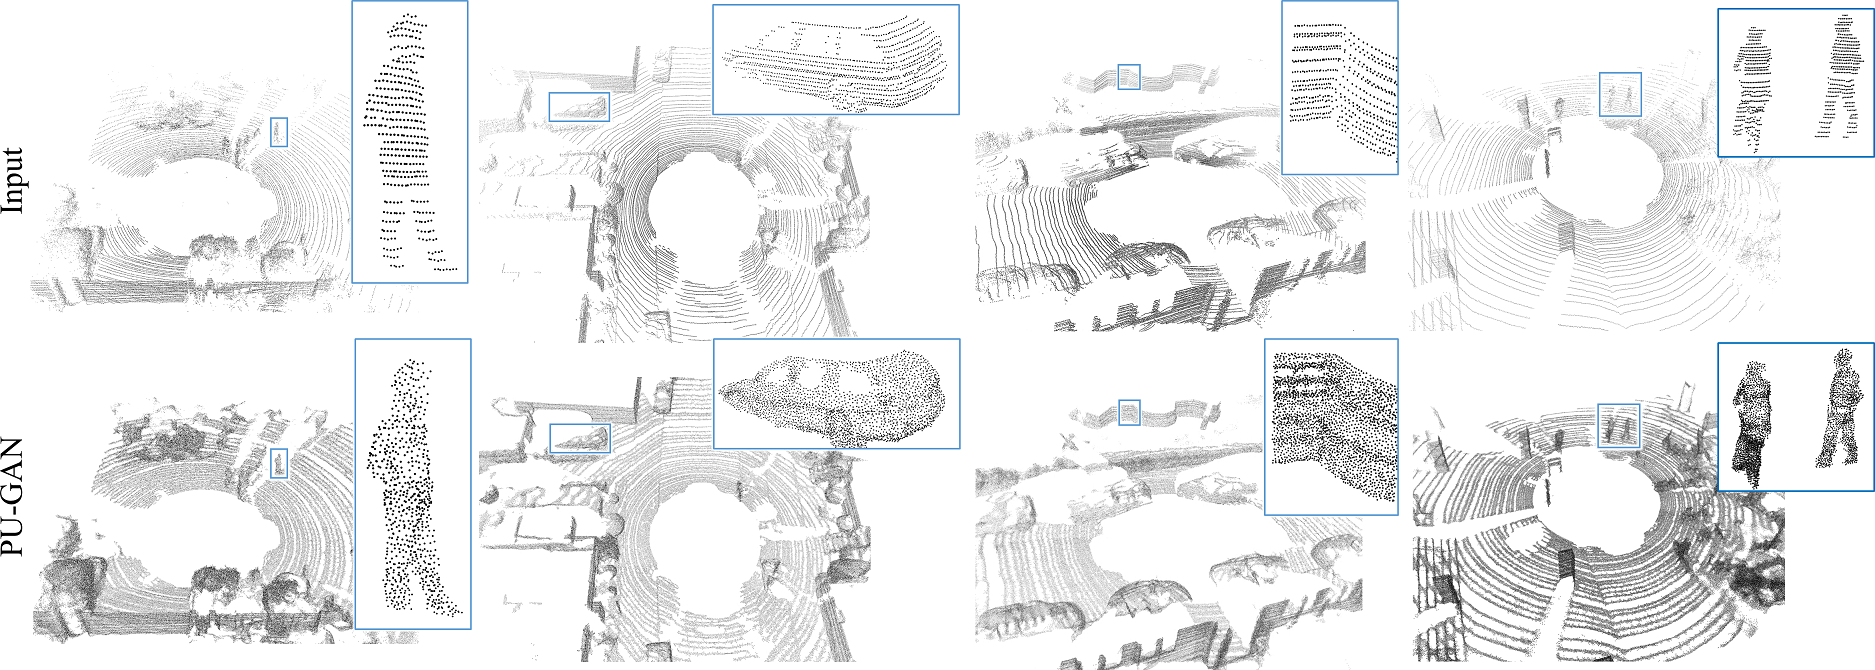
\includegraphics[width=1.0\linewidth]{realscan}
	\caption{Using PU-GAN to upsample real-scanned point cloud data acquired by LiDAR.}
	\label{fig:realscan}
	\vspace*{-2mm}
\end{figure*}



%%%%%%%%%%%%%%%%%%%%%%%%%%%%%%%%%%%%%%%%%%%%%%%%%%%%%%%%%%%



%%%%%%%%%%%%%%%%%%%%%%%%%%%%%%%%%%%%%%%%%%%%%%%%%%%%%%%%%%%

\subsection{Datasets and Implementation Details}
\label{subsec:dataset}
We collected 147 3D models from the released datasets of PU-Net~\cite{yu2018pu} and MPU~\cite{yifan2018patch}, as well as from the Visionair repository~\cite{visionair}, covering a rich variety of objects, ranging from simple and smooth models (\eg, Icosahedron) to complex and high-detailed objects (\eg, Statue); see the supplemental material for all of them.
Among them, we randomly select 120 models for training and use the rest for testing.
%We totally collect 147 models from the released datasets of PU-Net~\cite{yu2018pu} and MPU~\cite{yifan2018patch}, as well as the Visionair repository~\cite{visionair}, covering a variety of objects ranging from smooth and simple structures (\eg, Icosahedron) to complex and high-detailed objects (\eg, Statue); see the supplemental material for all the models.
%Among these models, we randomly select 120 for training and the rest 27 models for testing.

%On each patch, we employ Poisson disk sampling~\cite{corsini2012efficient} algorithm to generate 1,024 points as target uniform samples and then randomly select $N=256$ points on-the-fly from the sampled 1,024 points as inputs and feed them into the network for training.
%By default, the upsampling rate $r=4$.

%In the testing phase, we first use Poisson disk sampling to sample 8,192 points as ground truth on the object surface and then randomly select 2,048 points for testing.
%Note that, following MPU~\cite{yifan2018patch}, we also adopt the patch-based testing strategy.
%Specifically, we apply farthest sampling to select 24 seeds from the 2,048 points, and then grow a point subset at each seed with 256 points.
%We feed these point subsets into the generator for upsampling, and then combine the upsampled points together, apply the farthest sampling to get the final upsampled point cloud with 8,192 points.



%%%%%%%%%%%%%%%%%%%%%%%%%%%%%%%%%%%%%%%%%%%%%%%%%%%%%%%%%%%

%\subsection{Implementation Details}
%\label{subsec:implementation}

In the training phase, we cropped 200 patches per training model (see Section~\ref{subsubsec:train_data}) and produced $24,000$ patches in total.
By default, we set $N=256$, $r=4$, and $M=50$.
Moreover, for the uniform loss, we cropped one set of $S_j$ with radius $r_d=\sqrt{p}$ for each $p \in$ \{ 0.4\%, 0.6\%, 0.8\%, 1.0\%, 1.2\% \}, compute Eq.~\eqref{eq:uniform} five times for each set, and then sum up the results as the $\mathcal{L_{\text{uni}}}$ term in Eq.~\eqref{eq:compound}.

To avoid overfitting in training, we augment the network inputs by random rotation, scaling, and point perturbation with Gaussian noise.
%To calculate $\mathcal{L_{\text{uni}}}$ during training, we set the number of disks $M=50$.
We trained the network for 100 epochs using the Adam algorithm~\cite{kingma2014adam} with a two time-scale update rule (TTUR)~\cite{heusel2017gans}.
We set the learning rates of generator and discriminator as 0.001 and 0.0001, respectively; after 50k iterations, we gradually reduce both rates by a decay rate of 0.7 per 50k iterations until $10^{-6}$.
The batch size is 28, and $\lambda_{\text{rec}}$, $\lambda_{\text{uni}}$, and $\lambda_{\text{gan}}$ are empirically set as 100, 10, and 0.5, respectively.
We implemented our network using TensorFlow and trained it on NVidia Titan Xp GPU.

During the testing, given a point set, we follow the patch-based strategies in MPU~\cite{yifan2018patch} and EC-Net~\cite{yu2018ec} to use the farthest sampling to pick seeds and extract a local patch of $N$ points per seed.
Then, we feed the patches to the generator and combine the upsampled results as the final output.



%%%%%%%%%%%%%%%%%%%%%%%%%%%%%%%%%%%%%%%%%%%%%%%%%%%%%%%%%%%

\subsection{Evaluation Metrics}
\label{subsec:evaluation}
We employ four evaluation metrics: (i) uniformity using $\mathcal{L_{\text{uni}}}$ in Eq.~\eqref{eq:uniform}, (ii) point-to-surface (P2F) distance using the testing models, (iii) Chamfer distance (CD), and (iv) Hausdorff distance (HD)~\cite{berger2013benchmark}.
For quantitative evaluation, we use Poisson disk sampling to sample 8,192 points as the ground truth (\eg, see Figure~\ref{fig:visualComparison}(b)) on each of the testing models, and randomly select 2,048 points as testing input.
To evaluate the uniformity of the test results (using Eq.~\eqref{eq:uniform}), we randomly pick $M=1,000$ seeds on each result, and instead of using ball query to crop $S_j$, we use the actual mesh (testing model) to geodesically find $S_j$ at each seed of different $p$ for higher-quality evaluation.
The lower the metric values are, the better the upsampling results are.



%%%%%%%%%%%%%%%%%%%%%%%%%%%%%%%%%%%%%%%%%%%%%%%%%%%%%%%%%%%

\subsection{Qualitative and Quantitative Comparisons}
\label{subsec:comparison}

%\para{Comparison with state-of-the-arts.} \
We qualitatively and quantitatively compared PU-GAN with three state-of-the-art point set upsampling methods: EAR~\cite{huang2013edge}, PU-Net~\cite{yu2018pu}, and MPU~\cite{yifan2018patch}.
%Without additional surface and edge information, EC-Net\cite{yu2018ec} will degenerate into PU-Net.
For EAR, we employed the released demo code and generated the best results by exhaustively fine-tuning every associated parameter.
For PU-Net and MPU, we used their public code and retrained their networks using our training data.

Table~\ref{tab:quanComparison} shows the quantitative comparison results.
Our PU-GAN achieves the lowest values consistently for all the evaluation metrics.
Particularly, the uniformity of our results stays the lowest for all different $p$, indicating that the points generated by PU-GAN are much more uniform than those produced by others over varying scales.

Besides quantitative results, we show point set upsampling and surface reconstruction (using~\cite{kazhdan2013screened}) results for various models in Figure~\ref{fig:visualComparison}.
%The input point set has 2,048 non-uniform points and we upsample 4$\times$ for each approach.
%We reconstruct the surface from the point set by using the screened Poisson reconstruction algorithm~\cite{kazhdan2013screened}.
%Note that all the testing objects are different from the training objects.
Comparing the results produced by (f) our method and by (c-e) others, against (b) the ground truth points that are uniformly-sampled on the original testing models, we can see that other methods tend to produce more noisy and nonuniform point sets, thus leading to more artifacts in the reconstructed surfaces.
See, particularly, the blown-up views, showing that PU-GAN can produce more fine-grained details in the upsampled results,~\eg, elephant's nose (top) and tiger's tail (bottom).
%Hence, the reconstructed meshes by our PU-GAN are the closest to the ground truths.
More comparison results can be found in the supplemental material.

%For non-uniform consideration, we set a small $neighborhood \;  number = 10$ for PCA normal estimation\cite{hoppe1992surface} and $depth = 8$ for screened Possion reconstruction\cite{kazhdan2013screened}. As shown in Figure \ref{fig:visualComparison}, EAR maintains the upsampled points along the surface, but struggles with these regions of large gap. The non-uniform inputs have a huge negative impact on the performance of PU-Net, which tends to generate points around the original inputs. Instead of directly upsampling with 4 times, MPU can take advantage of all the intermediate multiples of data with a progressive training strategy. Based on that, MPU enables to fill more points in those non-contiguous areas but is difficult to produce clean and more well defined outputs. In comparison, our method is superior to all these methods quantitatively by a large margin. Qualitatively, our generated results are more uniform, less noisy and restore the underlying geometry.



%%%%%%%%%%%%%%%%%%%%%%%%%%%%%%%%%%%%%%%%%%%%%%%%%%%%%%%%%%%

\subsection{Upsampling Real-scanned Data}

Figure~\ref{fig:realscan} shows upsampling results on LiDAR point clouds (downloaded from KITTI dataset~\cite{geiger2013vision}) produced by PU-GAN.
From the first row, we can see the sparsity and non-uniformity of the inputs.
%Hence, it is quite challenging to upsample these points without any additional prior knowledge.\phil{hard to without prior knowledge... since the network also learns from the training set}
%Even under such case,
Our PU-GAN can still fill some holes and output more uniform points in the results; please see the supplemental material for more results.



\begin{table}[!t]
\centering
\caption{Quantitative comparisons with the state-of-the-arts.}
\label{tab:quanComparison}
\resizebox{\linewidth}{!}{
	\begin{tabular}{@{\hspace{1mm}}c@{\hspace{1mm}}||@{\hspace{1mm}}c@{\hspace{3mm}}c@{\hspace{3mm}}c@{\hspace{3mm}}c@{\hspace{3mm}}c@{\hspace{1mm}}|@{\hspace{0.2mm}}c@{\hspace{1mm}}|@{\hspace{1mm}}c@{\hspace{1mm}}|@{\hspace{1mm}}c@{\hspace{1mm}}} \toprule[1pt]
	\multirow{2}*{Methods} & \multicolumn{5}{@{\hspace{1mm}}c@{\hspace{1mm}}|@{\hspace{0.2mm}}}{Uniformity for different $p$ ($10^{-3}$)} & P2F & CD & HD \\ \cline{2-6}
	& 0.4\% & 0.6\% & 0.8\% & 1.0\% & 1.2\% & ($10^{-3}$) & ($10^{-3}$) & ($10^{-3}$)\\ \hline \hline
	EAR~\cite{huang2013edge}  &  16.84  & 20.27  & 23.98  &  26.15  & 29.18   & 5.82 & 0.52  & 7.37   \\
	PU-Net~\cite{yu2018pu} &  29.74  & 31.33  & 33.86  & 36.94   & 40.43 & 6.84 & 0.72  & 8.94   \\
	MPU~\cite{yifan2018patch} & 7.51  & 7.41  & 8.35  & 9.62   & 11.13  & 3.96 & 0.49  & 6.11   \\ \hline
	PU-GAN & \textbf{3.38} & \textbf{3.49}  & \textbf{3.44}  & \textbf{3.91}  & \textbf{4.64} & \textbf{2.33} & \textbf{0.28}  & \textbf{4.64}    \\ \bottomrule[1pt]
	\end{tabular}}
	%\vspace*{-2mm}
\end{table}

\begin{table}[t]
	\centering
	\caption{Quantitative comparisons:
		removing each specific component from the full PU-GAN pipeline (top five rows) vs. baseline GAN model (6-th row) vs. full PU-GAN pipeline (last row).}
	%	\caption{The upsampling results in terms of each evaluation metric when removing different component individually compared to our full pipeline, as well as the baseline results.}
	\label{tab:ablationStudy}
	\resizebox{\linewidth}{!}{
		\begin{tabular}{@{\hspace{1mm}}c@{\hspace{1mm}}||@{\hspace{1mm}}c@{\hspace{3mm}}c@{\hspace{3mm}}c@{\hspace{3mm}}c@{\hspace{3mm}}c@{\hspace{1mm}}|@{\hspace{0.2mm}}c@{\hspace{1mm}}|@{\hspace{1mm}}c@{\hspace{1mm}}|@{\hspace{1mm}}c@{\hspace{1mm}}} \toprule[1pt]
			\multirow{2}*{} & \multicolumn{5}{@{\hspace{1mm}}c@{\hspace{1mm}}|@{\hspace{0.2mm}}}{Uniformity for different $p$ ($10^{-3}$)} & P2F & CD & HD \\ \cline{2-6}
			& 0.4\% & 0.6\% & 0.8\% & 1.0\% & 1.2\% & ($10^{-3}$) & ($10^{-3}$) & ($10^{-3}$)\\ \hline \hline
			Discriminator       &  7.02  & 7.31  & 8.36  &  9.70  & 11.17  & 4.61 & 0.57  & 7.25  \\
			$\mathcal{L_{\text{uni}}}$ & 5.15  & 5.71  & 6.13  & 6.82   & 7.32  & 3.99 & 0.51  & 6.22  \\
			self-attention                &  4.19  & 4.66  & 4.87  & 5.52   & 6.47 & 3.97 & 0.46  & 6.01  \\
			up-down-up             &   3.89 & 4.16 & 4.63 & 5.14 & 5.89 & 3.02 & 0.35	& 5.15\\
			farthest samp.            & 3.56  & 3.76  & 3.78  & 4.15   & 4.97 & 2.72 & 0.31  & 4.96  \\ \hline
			baseline GAN & 8.12  & 8.18  & 8.76  & 9.89   & 11.32  & 4.79 & 0.59  & 7.31   \\ \hline
			full pipeline  & \textbf{3.38} & \textbf{3.49}  & \textbf{3.44}  & \textbf{3.91}  & \textbf{4.64} & \textbf{2.33} & \textbf{0.28}  & \textbf{4.64}  \\ \bottomrule[1pt]
	\end{tabular}}
	\vspace*{-2mm}
	%\vspace*{-10pt}
\end{table}

%%%%%%%%%%%%%%%%%%%%%%%%%%%%%%%%%%%%%%%%%%%%%%%%%%%%%%%%%%%

\subsection{Ablation Study and Baseline Comparison}
\label{subsec:ablation}

To evaluate the components in PU-GAN, including the GAN framework (\ie, remove the discriminator and keep only the generator), up-down-up expansion unit, self-attention unit, uniform loss, and farthest sampling, we removed each of them from the network and generated upsampling results for the testing models.
Table~\ref{tab:ablationStudy} shows the evaluation results.
Our full pipeline performs the best, and removing any component reduces the overall performance, meaning that each component contributes.
Particularly, removing the GAN framework (\ie, removing the discriminator) causes the largest performance drop, thereby showing the effectiveness of adversarial learning in the framework.

%\para{Comparison with a baseline.} \
%Since no prior works develop GAN models for point cloud upsampling and amendment, we thus design a basic GAN model as the baseline for comparison.
Further, we designed a GAN baseline for comparison by removing $\mathcal{L_{\text{uni}}}$, self-attention unit, up-down-up expansion unit, and farthest sampling altogether; see supplemental material for its architecture.
%Specifically, the generator only expands features by upsampling once without the self-attention unit and farthest sampling.
%In the discriminator, we also remove the self-attention unit; see supplemental material for the baseline architecture.
%During training, we only keep the adversarial and reconstruction losses.
Quantitative results shown in the second last row of Table~\ref{tab:ablationStudy} and a visual comparison example shown in Figure~\ref{fig:baseline} demonstrate that simply applying a basic GAN framework is insufficient for the upsampling problem; our adaptations to the GAN model plus the various formulations contribute to realizing a working GAN model.


%%%%%%%%%%%%%%%%%%%%%%%%%%%%%%%%%%%%%%%%%%%%%%%%%%%%%%%%%%%

\begin{figure}[!t]
	\centering
	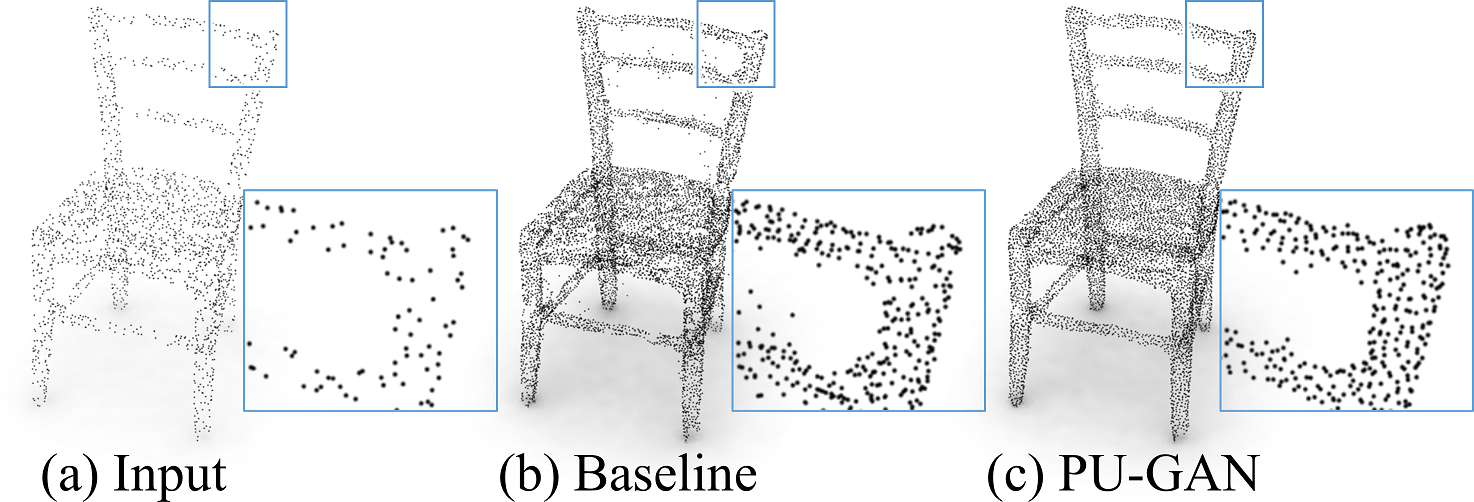
\includegraphics[width=1.0\linewidth]{baseline}
	\caption{Visual comparison of (c) PU-GAN against (b) the baseline GAN model, given (a) an input of 2,048 non-uniform points.}
	\label{fig:baseline}
	\vspace*{-2mm}
\end{figure}



%As Table ~\ref{tab:ablationStudy} shows, all components contributes positively to the full model. In particularly, the adversarial training can significantly boost the performance of upsampling procedure. Integrated attention module and uniform loss considerably promote the upsampling results and the farthest sampling improves performance slightly. After replacing the proposed up-down-up expansion unit with one up expansion, the uniformity of the generated points will be affected by a large negative impact.


\subsection{Other Experiments}

%\para{Upsampling with different noise levels.} \
%We investigate the robustness of PU-GAN by applying it to inputs of different noise levels.
%Figure~\ref{fig:noise} shows the comparison results with MPU~\cite{yifan2018patch}, where the inputs are corrupted by increasing amount of Gaussian noise, indicating that PU-GAN can still generate a satisfying upsampling result even under large noise corruption; see particularly the blown-up views.
%Please refer to our supplemental material for results under more continuous noise levels.
%can still generate a satisfying upsampling result even under large noise corruption.

\para{Upsampling point sets of varying noise levels.} \
Figure~\ref{fig:noise} shows the results of using PU-GAN to upsample point sets of increasing Gaussian noise levels, indicating the robustness of PU-GAN to noise and sparsity.
Please refer to the supplemental material for more results.

\para{Upsampling point sets of varying sizes.} \
Figure~\ref{fig:diff_point_num} shows the results of upsampling input point sets of different sizes; our method is stable even for input with only 512 points; more results are shown in the supplemental material.

\para{Applications.} \
Besides surface reconstruction and rendering (see Figure~\ref{fig:visualComparison}), point cloud upsampling is also helpful for object recognition.
To demonstrate this, we trained PointNet (vanilla version)~\cite{qi2016pointnet} on ModelNet40 dataset~\cite{wu20153d} for classification under two cases:
in case (i), we directly trained PointNet to take sparse training set (512 points) as inputs for classifying objects in the sparse testing set;
and in case (ii), we upsampled the point clouds in both sparse training and testing sets to 2,048 points using PU-GAN and then trained another PointNet with the upsampled training set for classifying the upsampled data in the testing set.
Results show that, the overall classification accuracy increased from 82.4\% (case (i)) to 83.8\% (case (ii)), indicating that PU-GAN helps improve the classification performance.


\begin{figure}[!t]
	\centering
	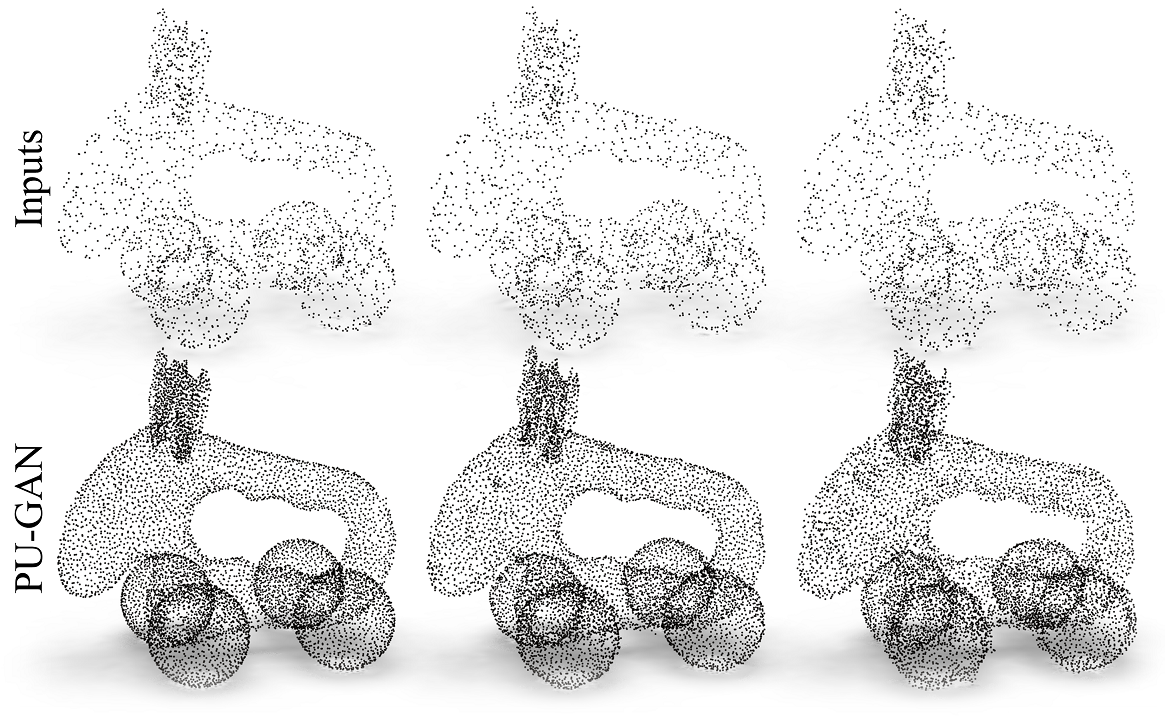
\includegraphics[width=1.0\linewidth]{noise}
	\vspace{-4mm}
	\caption{Upsampling results by applying PU-GAN to inputs with noise level of 0, 0.5\%, and 1\%.}
	\label{fig:noise}
	%\vspace*{-2mm}
\end{figure}

\begin{figure}[!t]
	\centering
	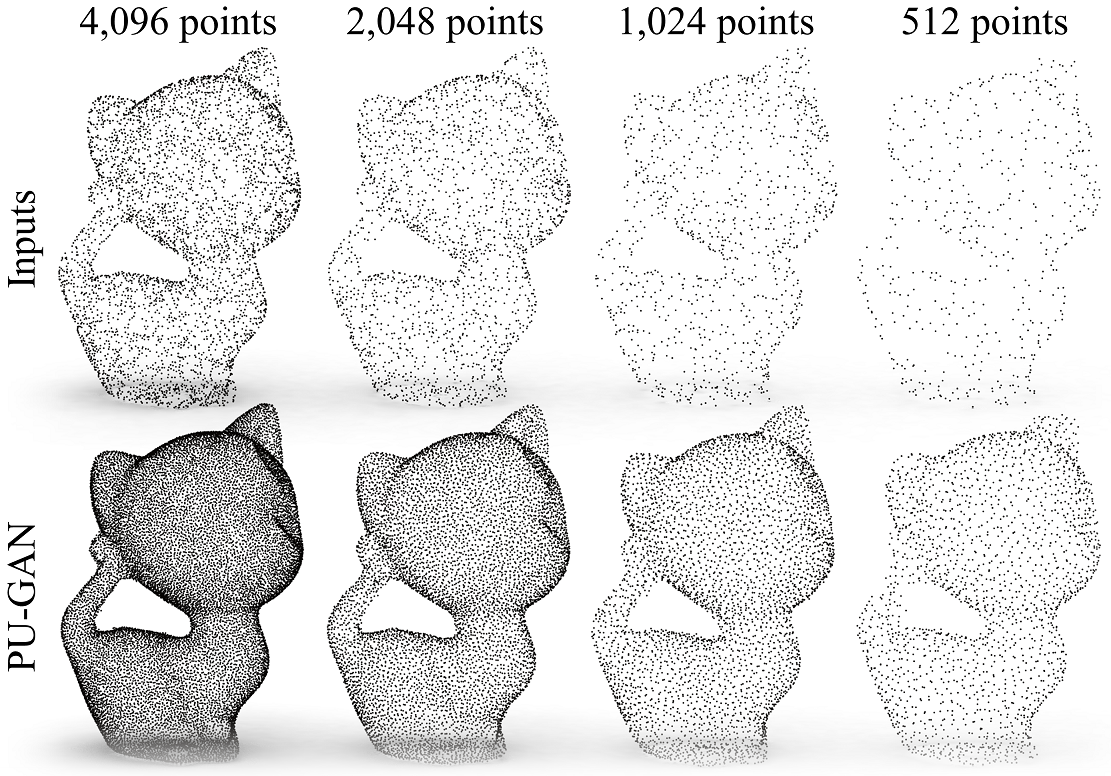
\includegraphics[width=1.0\linewidth]{diff_point_num}
	\vspace{-4mm}
	\caption{Upsampling point sets (top row) of varying sizes.} % 512,1024,2048,4096.}
	\label{fig:diff_point_num}
	\vspace*{-2mm}
\end{figure}


%\begin{table}[t]
%\centering
%	\caption{Classification accuracies by using PointNet on ModelNet40 dataset under case (i) with sparse point sets and case (ii) with our upsampled point sets.}
%	\label{tab:classification}
%\begin{tabular}{c|ccc}
%\toprule[1pt]
%ModelNet10                      & Case(i) & Case(ii) \\ \hline
%overall classification accuracy & 82.4\%    & 83.8\%     \\
%average class accuracy          & 76.7\%    & 77.8\%     \\
%\bottomrule[1pt]
%\end{tabular}
%\end{table}


\if 0
\subsection{Limitation}
\label{subsec:limitation}
As shown in Figure \ref{fig:limitation}, when there are some large gaps(\eg, head) among the given inputs, the proposed model just generate points around these holes, but can not fully complete the surface. And For which extremely sparse areas(\eg, foot), the produced results maybe noisy.

\begin{figure}
	\centering
	\includegraphics[width=1.0\linewidth]{limitation}
	\caption{Limitation for the proposed PU-GAN}
	\label{fig:limitation}
\end{figure}
\fi 